\documentclass[11pt,a4paper]{article}

\usepackage[margin=2.2cm]{geometry}
\usepackage[T1]{fontenc}
\usepackage[utf8]{inputenc}
\usepackage{lmodern}
\usepackage{amsmath,amssymb}
\usepackage{graphicx}
\usepackage{booktabs}
\usepackage{tabularx}
\usepackage{float}
\usepackage{caption}
\usepackage{enumitem}
\usepackage{xcolor}
\usepackage[hidelinks]{hyperref}

\graphicspath{{../figures/}{figures/}}
\setlist{itemsep=2pt, topsep=4pt}
\captionsetup{font=small, labelfont=bf}
\newcommand{\code}[1]{\texttt{#1}}

\title{\textbf{Learning to Rank on the Cranfield Collection}\\[4pt]
\large Information Retrieval --- Programming Assignment III}
\author{Group: Quad Query}
\date{}

\begin{document}
\maketitle

% ---------------------------------------------------------------------------
\section{Group details}

\begin{table}[H]
\centering
\begin{tabular}{ll}
\toprule
\textbf{Name} & \textbf{Roll number} \\
\midrule
Hrishikesh Tiwari & 22CH3FP39 \\
Shshank Mittal    & 22CS30051 \\
Rishit Garg       & 22CS30045 \\
Parth Patil       & 22CS30041 \\
\bottomrule
\end{tabular}
\end{table}

% ---------------------------------------------------------------------------
\section{Problem statement}

The goal is to learn ranking functions for the Cranfield collection from human relevance
judgments, instead of tuning them by hand. The collection has 1400 abstracts from
aeronautics, 225 queries and graded relevance judgments. The learned rankers are evaluated
on held-out queries with precision, recall and F1. The assignment asks for two methods:

\begin{itemize}
  \item \textbf{Method A: Boolean weighted zone scoring.} A document's score is a weighted
  sum of Boolean match scores over its zones (title, author, bibliography, body):
  \begin{equation}
    \text{score}(d,q) = \sum_{i=1}^{4} g_i\, s_i(d,q), \qquad g_i \in [0,1],\quad \sum_i g_i = 1 .
  \end{equation}
  The weights $g_i$ are learned by grid search from the relevance judgments.

  \item \textbf{Method B: real-valued weights with a linear SVM.} Each query--document pair
  is described by a feature vector $\psi(d,q)$, using the LETOR feature list given in the
  assignment. A linear SVM learns a weight vector $\mathbf{w}$, and documents are ranked by
  $\mathbf{w}^\top\psi(d,q)$.
\end{itemize}

For each test query, the system outputs a ranked list of documents and the set of documents
it considers relevant (the top $k$ of the list). Both are evaluated against the human
judgments.

% ---------------------------------------------------------------------------
\section{Implementation details}

The system is written in Python~3. It uses \code{numpy} for all index and feature
computation, \code{scikit-learn} for the SVM (\code{LinearSVC}) and \code{nltk} only for the
Porter stemmer. Table~\ref{tab:files} shows the code layout.

\begin{table}[H]
\centering
\small
\begin{tabularx}{\linewidth}{lX}
\toprule
\textbf{File} & \textbf{Contents} \\
\midrule
\code{src/parser\_qq.py}       & parsers for \code{cran.all.1400}, \code{cran.qry}, \code{cranqrel} \\
\code{src/preprocessing.py}    & tokenising, stopword removal, Porter stemming \\
\code{src/dataset.py}          & term-count matrix per zone, idf, ranking helper, query splits \\
\code{src/evals.py}            & P/R/F1@$k$, MAP, nDCG@10, cut-off tuning, TREC run files \\
\code{src/method\_a/}          & Boolean zone scores and grid search of zone weights \\
\code{src/method\_b/}          & 66 query--document features and linear SVM training \\
\code{main.py}                 & all experiments; ranking of unseen queries with the final models \\
\code{report/make\_figures.py} & figures from \code{results/summary.json} \\
\bottomrule
\end{tabularx}
\caption{Code layout.}
\label{tab:files}
\end{table}

\subsection{Data and preprocessing}

\begin{itemize}
  \item \textbf{Zones.} The document fields \code{.T}, \code{.A}, \code{.B} and \code{.W}
  become the zones \emph{title}, \emph{author}, \emph{bib} and \emph{body}. A fifth stream,
  \emph{all}, is the four zones joined together.

  \item \textbf{Query numbering.} The \code{.I} numbers in \code{cran.qry} are not
  $1,\dots,225$ (some values are skipped). \code{cranqrel} refers to queries by their
  \emph{position} in the file, so queries are numbered $1,\dots,225$ in the order they
  appear.

  \item \textbf{Placeholder judgments.} \code{cranqrel} has one line per query with code
  $-1$. These are placeholders, not judgments, and are dropped. That leaves 1612 judgments
  with codes 1--4, about 7.2 relevant documents per query.

  \item \textbf{Text processing.} Text is lowercased and split into alphanumeric tokens.
  Stopwords and one-letter tokens are removed, and the remaining tokens are Porter-stemmed,
  giving 6588 distinct stems. Queries go through the same pipeline, and a repeated query term
  is counted once. Queries average about 10 stems.

  \item \textbf{Index.} Each zone is stored as a dense term $\times$ document count matrix
  ($6588 \times 1400$). The features of a query are then numpy operations on the rows of its
  terms, and features for all 225 queries are computed in a few seconds. The idf is
  $\log\frac{N+1}{\text{df}+0.5}$.

  \item \textbf{Relevance.} Any judged document (codes 1--4) is relevant, and every other
  document is non-relevant. Where graded relevance is used (Ranking SVM, nDCG), the gain is
  $5-\text{code}$: 4 for ``complete answer'' down to 1 for ``minimum interest'', and 0 for
  unjudged documents.
\end{itemize}

\subsection{Method A: Boolean weighted zone scoring}

\paragraph{Boolean match functions.} Two Boolean functions $s_i(d,q)$ are compared:
\begin{itemize}
  \item \textbf{or} (the textbook definition): $s_i = 1$ if \emph{any} query term occurs in
  zone $i$, and 0 otherwise.
  \item \textbf{term} (per-term Boolean): with $s_i(t)=1$ if term $t$ occurs in zone $i$,
  \begin{equation}
    s_i(d,q) = \frac{1}{|q|}\sum_{t\in q} s_i(t),
  \end{equation}
  the fraction of query terms present in the zone. This is ranked Boolean matching applied
  one term at a time. It still uses only presence or absence, never frequencies, but a
  document that matches more query terms scores higher.
\end{itemize}

\paragraph{Grid search.} The weights are found by exhaustive search over every weight
vector on the 4-dimensional simplex with step 0.05, which gives 1771 candidates. Two
objectives are compared:
\begin{itemize}
  \item \textbf{mse} (the lecture formulation). Relevant documents are quantised as $r=1$
  and non-relevant ones as $r=0$, and the total squared error is minimised:
  \begin{equation}
    \varepsilon(g) = \sum_j \bigl(r(d_j,q_j) - \text{score}(d_j,q_j)\bigr)^2 .
  \end{equation}
  The training triples are every relevant document of each training query, plus three
  sampled non-relevant documents per relevant one. Negatives are sampled only from documents
  that match at least one query term, because a document with no match scores 0 under every
  $g$ and adds nothing to the search.
  \item \textbf{map}. The objective is the mean average precision of the ranking that $g$
  produces on the training queries. This optimises the ranking directly. All 1771
  candidates are evaluated together in vectorised form, and ties count as half a rank.
\end{itemize}
Ties in the final ranking are broken by document id.

\subsection{Method B: real-valued weights with a linear SVM}

\paragraph{Features.} All 22 features from the assignment are computed for each of three
streams: title, body and the whole document. That gives $22 \times 3 = 66$ features per
query--document pair. In Table~\ref{tab:features}, $\text{tf}_t$ is the count of query term
$t$ in the stream, $L$ is the stream length, and the aggregates are taken over the query
terms.

\begin{table}[H]
\centering
\small
\begin{tabularx}{\linewidth}{llX}
\toprule
\textbf{\#} & \textbf{Feature} & \textbf{Definition} \\
\midrule
1      & query term number                 & number of query terms present in the stream \\
2      & query term ratio                  & feature 1 divided by $|q|$ \\
3      & stream length                     & $L$ (tokens after preprocessing) \\
4      & idf                               & $\sum$ idf$(t)$ over query terms present in the stream \\
5--9   & tf: sum, min, max, mean, variance & aggregates of $\text{tf}_t$ \\
10--14 & normalised tf: sum \dots\ variance & aggregates of $\text{tf}_t / L$ \\
15--19 & tf$\cdot$idf: sum \dots\ variance & aggregates of $\text{tf}_t \cdot \text{idf}(t)$ \\
20     & Boolean model                     & 1 if any query term is present \\
21     & vector space model                & cosine of the $(1+\log \text{tf})\cdot$idf document vector and the idf query vector \\
22     & BM25                              & Okapi BM25 with $k_1 = 1.2$, $b = 0.75$ \\
\bottomrule
\end{tabularx}
\caption{Features per stream (the list from the assignment).}
\label{tab:features}
\end{table}

The ``idf'' feature is summed only over the query terms that occur in the document. In LETOR
it is the sum over all query terms, which is the same for every document of a query and would
become 0 after per-query normalisation. The Boolean model uses ``any term matches'', because
an ``all terms match'' version is 0 for almost every document when queries have about 10
terms. Every feature is min--max normalised \emph{per query} (LETOR ``QueryLevelNorm''), so
each weight compares documents of the same query.

\paragraph{Learning.} Two linear SVM formulations are trained with \code{LinearSVC} (hinge
loss with L2 regularisation):
\begin{itemize}
  \item \textbf{Pointwise SVM.} Each pair $(\psi(d,q), \text{relevant or not})$ is one
  training example. Only about 0.5\% of the pairs are relevant, so class weights are
  balanced. Documents are ranked by $\mathbf{w}^\top\psi + b$.
  \item \textbf{Pairwise Ranking SVM.} For two documents of the same query with different
  grades, the difference vector
  \begin{equation}
    \Phi(d_i,d_j,q) = \psi(d_i,q) - \psi(d_j,q)
  \end{equation}
  is labelled $+1$ if $d_i$ is more relevant and $-1$ otherwise. The grades give the order
  code $1 \succ 2 \succ 3 \succ 4 \succ$ unjudged. At most 2000 pairs are sampled per query,
  and half of them have their sign flipped so that both classes are present. The SVM has no
  intercept, and documents are ranked by $\mathbf{w}^\top\psi$.
\end{itemize}
Every document in the collection is scored. The regularisation parameter $C$ is chosen from
$\{10^{-4}, 10^{-3}, 10^{-2}, 10^{-1}, 1\}$ by 5-fold cross-validation \emph{on the training
queries}, with MAP as the criterion. The test queries are never used for model selection.

\subsection{Output and evaluation}

\begin{itemize}
  \item For each test query, the top 100 documents are written in TREC format
  (\code{qid Q0 docid rank score tag}) to \code{results/method\_*\_test\_results.txt}.
  \item The documents returned as relevant are the top $k$ of the ranking, where $k$ is the
  value in $1,\dots,50$ that maximises mean F1@$k$ on the \emph{training} queries. These
  result sets are in \code{results/method\_*\_test\_relevant.txt}.
  \item Measures are averaged over queries: precision, recall and F1 at $k = 5, 10, 20$ and
  at the tuned $k$. MAP and nDCG@10 (graded) are reported as additional measures of ranking
  quality.
  \item \code{python main.py predict A|B <queries> <out>} ranks unseen queries with the
  final models, which are retrained on all 225 queries.
\end{itemize}

% ---------------------------------------------------------------------------
\section{Plan of experiments}

\begin{enumerate}
  \item \textbf{Split.} The 225 judged queries are shuffled with a fixed seed (42) and split
  70/30 into 157 training and 68 test queries. All learning, including the weights, $C$ and
  the cut-off $k$, uses only the training queries.
  \item \textbf{Method A.} Two Boolean functions (or, term) $\times$ two objectives (mse,
  map). The learned weights and the objective along the grid are inspected, and each variant
  is evaluated on the test queries.
  \item \textbf{Method B.} The pointwise SVM and the Ranking SVM, each with $C$ chosen by
  inner cross-validation, are evaluated on the test queries. The learned feature weights are
  inspected.
  \item \textbf{Baseline.} BM25 on the whole document, which is the strongest hand-built
  ranker that the same features can provide.
  \item \textbf{Robustness.} 5-fold cross-validation over all 225 queries for the main
  systems, to check that the result on a single split holds.
  \item \textbf{Final models.} The chosen configurations are retrained on all 225 queries
  (\code{models/*.json}) and used to rank the unknown test queries.
  \item \textbf{Extra checks.} Log-transformed and z-scored features instead of min--max,
  and 8000 instead of 2000 pairs per query.
\end{enumerate}

% ---------------------------------------------------------------------------
\section{Results}

\subsection{Held-out test queries}

\begin{table}[H]
\centering
\small
\begin{tabular}{lcccccccc}
\toprule
\textbf{Run} & \textbf{P} & \textbf{R} & \textbf{F1} & \textbf{P@10} & \textbf{R@10} & \textbf{F1@10} & \textbf{MAP} & \textbf{nDCG@10} \\
\midrule
A or / mse            & 0.0235 & 0.1038 & 0.0371 & 0.0368 & 0.0737 & 0.0472 & 0.0595 & 0.0489 \\
A or / map            & 0.0294 & 0.1163 & 0.0438 & 0.0456 & 0.0963 & 0.0588 & 0.0704 & 0.0613 \\
A term / mse          & 0.1891 & 0.2606 & 0.1984 & 0.1559 & 0.2908 & 0.1844 & 0.2241 & 0.2770 \\
\textbf{A term / map} & 0.1868 & 0.3488 & 0.2211 & 0.1868 & 0.3488 & 0.2211 & 0.2701 & 0.3371 \\
\midrule
B pointwise SVM       & 0.2710 & 0.3485 & 0.2739 & 0.2265 & 0.4097 & 0.2644 & 0.3194 & 0.3938 \\
\textbf{B Ranking SVM}& \textbf{0.2815} & \textbf{0.3618} & \textbf{0.2853} & \textbf{0.2294} & \textbf{0.4131} & \textbf{0.2675} & \textbf{0.3245} & \textbf{0.3991} \\
\midrule
BM25 baseline         & 0.2689 & 0.3464 & 0.2749 & 0.2235 & 0.3939 & 0.2608 & 0.3148 & 0.3832 \\
\bottomrule
\end{tabular}
\caption{Results on the 68 test queries. P, R and F1 (without @) are for the set of
documents returned as relevant, i.e.\ the top $k$, where $k$ is tuned on the training
queries for each run ($k=10$ for A term/map; $k=7$ for Method B and BM25). Bold rows are
the final configuration of each method.}
\label{tab:test}
\end{table}

\begin{table}[H]
\centering
\small
\begin{tabular}{lcccccc}
\toprule
\textbf{Run} & \textbf{P@5} & \textbf{R@5} & \textbf{F1@5} & \textbf{P@20} & \textbf{R@20} & \textbf{F1@20} \\
\midrule
Method A (term / map)   & 0.2588 & 0.2642 & 0.2368 & 0.1294 & 0.4500 & 0.1864 \\
Method B pointwise SVM  & 0.3206 & 0.3099 & 0.2837 & 0.1529 & 0.5219 & 0.2190 \\
Method B Ranking SVM    & 0.3324 & 0.3148 & 0.2906 & 0.1544 & 0.5277 & 0.2213 \\
BM25 baseline           & 0.3118 & 0.3059 & 0.2796 & 0.1456 & 0.5003 & 0.2090 \\
\bottomrule
\end{tabular}
\caption{Precision, recall and F1 at cut-offs 5 and 20 on the test queries.}
\label{tab:test2}
\end{table}

\begin{figure}[H]
\centering
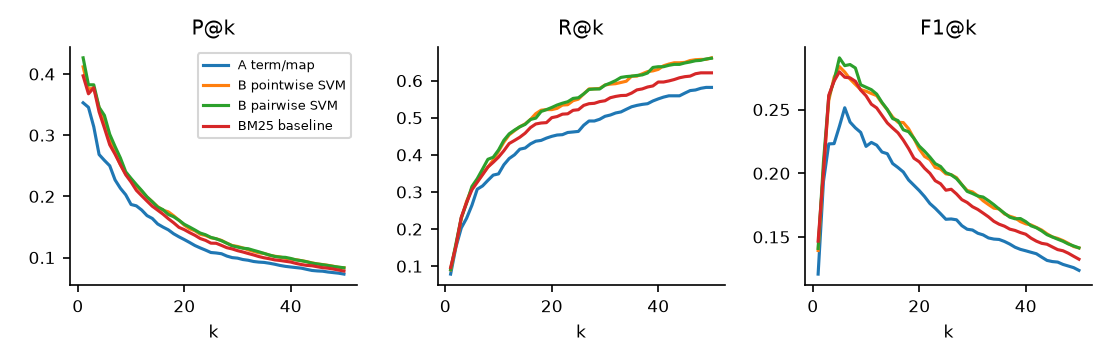
\includegraphics[width=\linewidth]{prf_curves.png}
\caption{Precision, recall and F1 against the cut-off $k$ on the test queries.}
\label{fig:prf}
\end{figure}

\subsection{Cross-validation over all queries}

\begin{table}[H]
\centering
\small
\begin{tabular}{lc}
\toprule
\textbf{System} & \textbf{5-fold CV MAP} \\
\midrule
Method A (term / map)  & 0.2738 \\
Method B pointwise SVM & 0.3273 \\
Method B Ranking SVM   & 0.3260 \\
BM25 baseline          & 0.3192 \\
\bottomrule
\end{tabular}
\caption{MAP averaged over five query folds covering all 225 judged queries.}
\label{tab:cv}
\end{table}

\subsection{Method A: learned zone weights}

\begin{table}[H]
\centering
\small
\begin{tabular}{lcccc}
\toprule
\textbf{Variant} & $g_\text{title}$ & $g_\text{author}$ & $g_\text{bib}$ & $g_\text{body}$ \\
\midrule
or / mse   & 0.40 & 0.40 & 0.15 & 0.05 \\
or / map   & 0.20 & 0.10 & 0.05 & 0.65 \\
term / mse & 0.20 & 0.00 & 0.00 & 0.80 \\
term / map & 0.50 & 0.05 & 0.00 & 0.45 \\
\bottomrule
\end{tabular}
\caption{Zone weights learned on the 157 training queries (grid step 0.05). Retraining
term/map on all 225 queries gives the same weights.}
\label{tab:weightsA}
\end{table}

\begin{figure}[H]
\centering
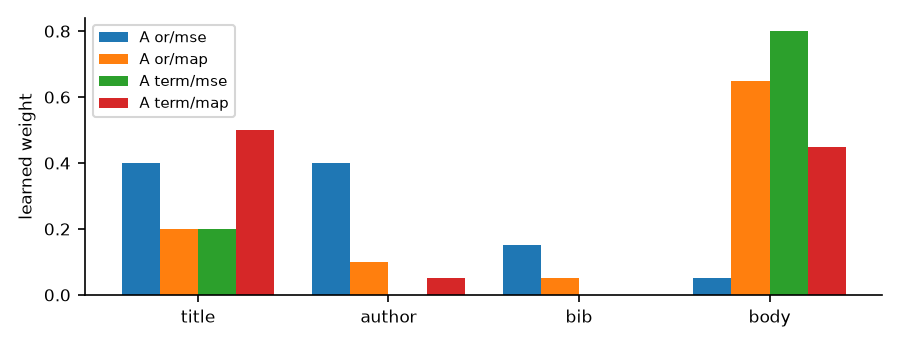
\includegraphics[width=0.7\linewidth]{method_a_weights.png}
\caption{Learned zone weights for the four Method A variants.}
\label{fig:weightsA}
\end{figure}

\begin{figure}[H]
\centering
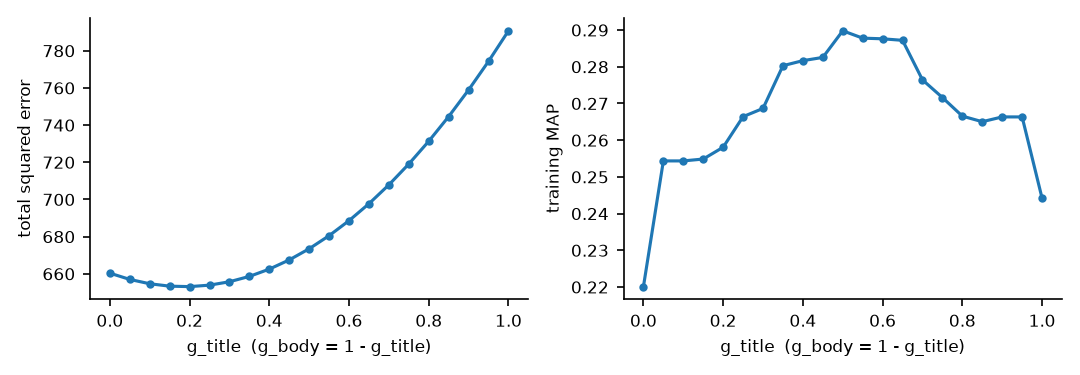
\includegraphics[width=0.95\linewidth]{method_a_grid.png}
\caption{Training objectives for the per-term Boolean function along the title/body edge of
the simplex ($g_\text{author}=g_\text{bib}=0$, $g_\text{body}=1-g_\text{title}$). This is
the four-zone version of choosing $g$ in the two-zone example from the lecture. Left:
total squared error (lower is better). Right: training MAP (higher is better).}
\label{fig:grid}
\end{figure}

\subsection{Method B: model selection and learned weights}

Inner 5-fold cross-validation on the training queries gave the following MAP for each $C$:

\begin{table}[H]
\centering
\small
\begin{tabular}{lccccc}
\toprule
$C$ & $10^{-4}$ & $10^{-3}$ & $10^{-2}$ & $10^{-1}$ & $1$ \\
\midrule
Pointwise SVM & \textbf{0.3303} & 0.3207 & 0.3182 & 0.3170 & 0.3153 \\
Ranking SVM   & \textbf{0.3290} & 0.3284 & 0.3211 & 0.3156 & 0.3137 \\
\bottomrule
\end{tabular}
\caption{Inner cross-validation MAP for each $C$. $C=10^{-4}$ was chosen for both SVMs.}
\label{tab:C}
\end{table}

\begin{figure}[H]
\centering
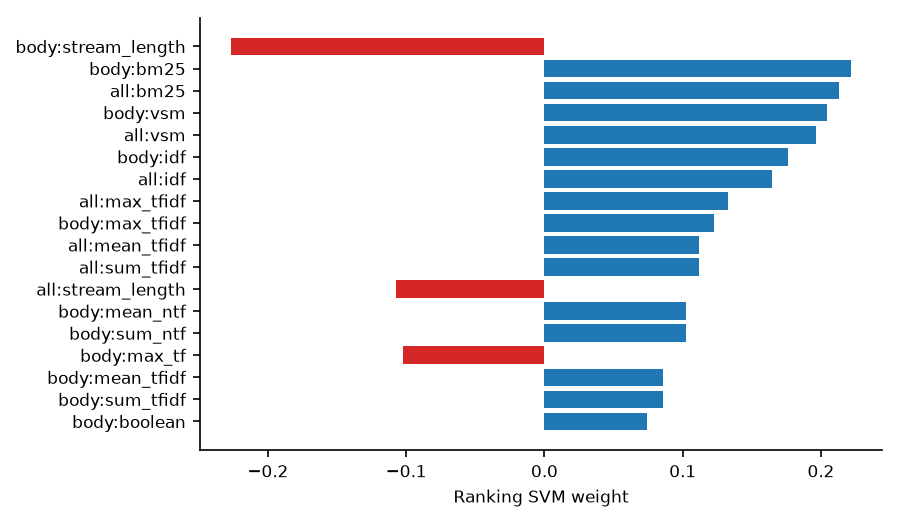
\includegraphics[width=0.75\linewidth]{method_b_weights.png}
\caption{The 18 largest-magnitude weights of the Ranking SVM. Features are normalised per
query, so the weights can be compared directly. Blue: positive. Red: negative.}
\label{fig:weightsB}
\end{figure}

\begin{figure}[H]
\centering
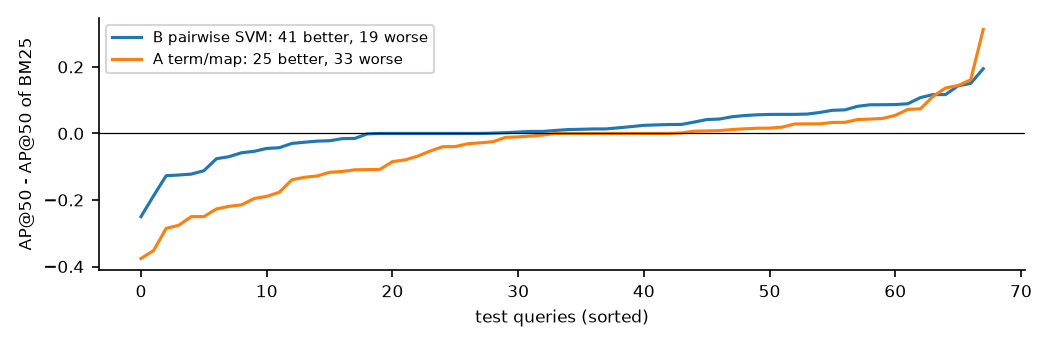
\includegraphics[width=0.9\linewidth]{per_query_ap.png}
\caption{Per-query difference in AP (top 50) from the BM25 baseline on the test queries,
sorted. The Ranking SVM beats BM25 on 41 queries and loses on 19. Method A beats it on 25
and loses on 33.}
\label{fig:perq}
\end{figure}

% ---------------------------------------------------------------------------
\section{Discussion of results}

\subsection{Method A}

\paragraph{The textbook ``any term'' Boolean function does not work on Cranfield.} Its test
MAP is only 0.070. Cranfield queries are long natural-language questions, about 10 stems
after stopword removal. Almost every document matches some query term in its body, and many
match in the title too. With four Boolean zones, the score can take only $2^4 = 16$ values,
so the ranking is mostly a large tie broken by document id. The learned weights are also
unstable. Under mse, author and bibliography get large weights (0.40 and 0.15): those zones
almost never match, and a score of 0 is the ``correct'' prediction for most of the
non-relevant training examples.

\paragraph{Counting matched terms per zone fixes this.} The per-term Boolean function still
uses only presence and absence, but it counts how many query terms each zone covers. Test
MAP rises from 0.070 to 0.270 and F1@10 from 0.059 to 0.221.

\paragraph{The learned weights are easy to interpret.} Title and body carry almost all of
the weight, and author and bibliography get about 0, because queries never mention authors
or journals. Under the MAP objective the title gets about half of the weight, even though in
Cranfield the abstract repeats the title. A title match is a strong signal for such a short
field.

\paragraph{The squared-error objective and the ranking objective disagree.} mse chooses
$(g_\text{title}, g_\text{body}) = (0.20, 0.80)$, while MAP chooses $(0.50, 0.45)$.
Squared error asks the score to \emph{equal} 0 or 1, which a convex combination of match
fractions cannot do, and the many negatives dominate it. Ranking only needs relevant
documents to score \emph{higher} than non-relevant ones. The MAP objective does better on
the test queries (MAP 0.270 vs.\ 0.224, F1 0.221 vs.\ 0.198). This illustrates the lecture's
point that ranking is better treated as ordinal regression than as classification or
regression. Fig.~\ref{fig:grid} also shows that the MAP landscape is flat for
$g_\text{title} \in [0.35, 0.65]$, so the coarse grid used in the lecture would find
essentially the same optimum.

\paragraph{Method A stays below BM25} (MAP 0.270 vs.\ 0.315). Presence and absence cannot
express term frequency, document length or term rarity (idf), which are exactly what BM25
adds.

\subsection{Method B}

\paragraph{The Ranking SVM is the best system on the test queries.} It reaches MAP 0.325,
nDCG@10 0.399 and F1 0.285 at the tuned cut-off, against 0.315, 0.383 and 0.275 for BM25. It
improves AP on 41 of the 68 test queries and hurts 19 (Fig.~\ref{fig:perq}). In
cross-validation over all queries, both SVMs again beat BM25, by about 0.007--0.008 MAP
(Table~\ref{tab:cv}).

\paragraph{The gain over BM25 is small, and that is expected.} All 66 features are functions
of the same query-term statistics, and BM25 already combines tf, idf and document length in
a well-tuned non-linear way. The learned model (Fig.~\ref{fig:weightsB}) amounts to: use
BM25 and the vector-space score on the body and the whole document, reward documents that
match rare query terms (the idf of matched terms) and that have a high maximum tf$\cdot$idf,
and penalise long documents. A linear SVM can only re-weight evidence that BM25 already
uses. Larger gains would need different evidence, such as term proximity, phrase matches or
query expansion, which the feature list does not contain. The extra checks support this:
log or z-score normalisation and more pairs per query all changed cross-validation MAP by
less than 0.005. The limit is the feature set, not the optimiser.

\paragraph{Pairwise vs.\ pointwise.} The Ranking SVM uses the graded judgments and only has
to order documents within a query, so it should have an advantage. It wins on the test split
(MAP 0.325 vs.\ 0.319, F1 0.285 vs.\ 0.274), but in cross-validation the two are tied
(0.3260 vs.\ 0.3273). Per-query normalisation already removes most of the differences
between queries that pairwise learning is meant to handle, and binary relevance carries most
of the signal on this collection.

\paragraph{Strong regularisation helps.} Both SVMs chose the smallest $C$ tried
($10^{-4}$), and MAP drops steadily as $C$ grows (Table~\ref{tab:C}). With about 150
training queries and highly correlated features (tf, normalised tf, tf$\cdot$idf and BM25 of
the same stream), a small $C$ spreads the weight across correlated features instead of
fitting noise. Since the optimum is at the edge of the grid, a slightly smaller $C$ might
help a little. The curve is already flattening, so we expect the difference to be small.

\subsection{Precision, recall and the cut-off}

Cranfield queries have about 7 relevant documents each, so as $k$ grows, precision falls
quickly and recall rises (Fig.~\ref{fig:prf}). F1 peaks at a small $k$. The cut-off tuned on
the training queries ($k=7$ for Method B) gives test precision 0.282, recall 0.362 and F1
0.285: about two of the seven returned documents are relevant. The absolute numbers are
modest because Cranfield is hard for lexical matching (abstracts often paraphrase the
question in other technical terms) and because ``minimum interest'' documents (code 4) also
count as relevant.

\subsection{Conclusion}

Both methods learn sensible weights from the relevance judgments. For Boolean zone scoring,
the choice of Boolean function and of a ranking-aware objective matters far more than the
grid resolution, and the learned weights confirm that title and body carry the evidence. The
Ranking SVM on the LETOR features gives the best results and beats the strongest hand-built
baseline (BM25) consistently, though only slightly. Pairwise and pointwise SVMs perform
about the same.

% ---------------------------------------------------------------------------
\appendix
\section{How to run}

\begin{verbatim}
python3 -m venv irenv
source irenv/bin/activate
pip install -r requirements.txt

python main.py                                  # all experiments (8-10 min)
python main.py predict B queries.qry run_B.txt  # rank unseen queries
python report/make_figures.py                   # regenerate figures/
\end{verbatim}

\noindent The query file for \code{predict} must be in Cranfield format (\code{.I} and
\code{.W} lines). Queries are numbered by their order in the file. The output is the top 100
documents per query in TREC format. Full instructions are in \code{README.md}.

\end{document}
